\documentclass[11pt,a4paper]{article}

% ============================================================
%  Revised Master's Project Report
%  Revision addresses the supervisor's review comments.
%  See accompanying "Summary of Revisions" for a comment-by-comment map.
% ============================================================

\usepackage[a4paper,margin=1in]{geometry}
\usepackage[T1]{fontenc}
\usepackage[utf8]{inputenc}
\usepackage{graphicx}
\usepackage{amsmath,amssymb}
\usepackage{booktabs}
\usepackage{multirow}
\usepackage{array}
\usepackage{url}
\usepackage{hyperref}
\usepackage{float}
\usepackage{setspace}
\usepackage{caption}

\graphicspath{{figures/}{analysis/plots/}{results/plots/}{./}}
\setstretch{1.08}
\hypersetup{colorlinks=true,linkcolor=blue,citecolor=blue,urlcolor=blue}

\title{A Unified FIDE, Chess.com, and Lichess Database:\\
Analyzing Elite Chess Players and their Behavioral Patterns}

\author{%
Ajay~Sathish~Shenoy,~24-745-606 \and
Ved~Chintamni~Bhatawadekar,~25-744-806 \and
Tony~Kristic,~24-754-004%
}
\date{%
Supervisors: Prof.\ Dr.\ Anik\'o Hann\'ak, Prof.\ Dr.\ Christoph Stadtfeld\\[2pt]
MSc Informatics, University of Zurich, Zurich, Switzerland}

\begin{document}

\maketitle

\begin{abstract}
This report introduces a unified database of elite chess players built from three
fundamental sources --- FIDE, Chess.com, and Lichess --- and uses it to study behavioral
patterns in online chess. Building this database is the central contribution and the main
research challenge of the project: official over-the-board (FIDE) identities and online
playing accounts are stored in incompatible formats, exposed through different access
channels, and rarely share an explicit key. The motivation for unifying them is to let
researchers translate existing ``over-the-board'' findings to online chess at scale. To
demonstrate the value of the database, we pursue two research questions that share the
same linked identities but probe different behaviors. The first is \emph{behavioral and
social}: do players behave differently (in game length / resignation and opening posture)
when facing female opponents, where the opponent's gender is established through the
FIDE-linked identity layer? The second is \emph{strategic}: which factors --- player
strength, activity, and gender --- shape a player's opening repertoire and its diversity?
The two questions are connected by the database itself: the same FIDE-anchored identity
map that lets us assign opponent gender also lets us measure each player's repertoire over
their full online game history. We report statistically detectable but small game-length
differences by opponent-gender context (and confirm that absolute rating difference, not
signed rating difference, is the relevant control), and a strong link between opening
diversity and player activity/strength. We present full regression tables, discuss the low
explanatory power of the behavioral model, and outline the limitations of perceived-gender
inference.
\end{abstract}

\noindent\textbf{Keywords:} data scraping, record linkage, big data, gender effects,
opening repertoire, data integration, behavioral modeling, regression analysis.

% ============================================================
\section{Introduction}
% ============================================================
There are sports in which players do not start from identical conditions. Chess, by
contrast, is usually regarded as exceptionally fair: the only structural asymmetry is that
White has a small first-move advantage in the opening phase. Tournament formats try to
balance this. In a round-robin event each player receives an (almost) equal number of games
with White and Black. In the Swiss system --- by far the most common format for open
tournaments --- colours are balanced as far as possible across a player's games, but an
exactly equal split is not guaranteed. Either way, the rules themselves do not favour any
participant.

Equal rules, however, do not imply equal behavioral dynamics. Chess has strong
psychological dimensions --- expectations about the opponent, opening preparation, and
social context --- that influence decision-making during a game and have deeper
implications for player behavior. One of the most debated questions in the chess world is
whether women-only titles (WGM, WIM, \dots) motivate female players or instead constrain
their perceived potential~\cite{maass2008checkmate}. With the rise of online chess and the
impact of strong engines on opening theory, the psychology of competitive chess has evolved
further over the past decade. Yet academic research has focused almost entirely on
``over-the-board'' (OTB) chess~\cite{bilalic2009why,blanch2017sex,backus2023gender}, and
online and OTB activity have not been analyzed together in a unified way.

\paragraph{The data-integration research challenge.}
Closing that gap is not only an analysis task --- it is a data-engineering and record-linkage
research challenge, and it is the part of this project that required the most effort. FIDE,
Chess.com, and Lichess describe the \emph{same} elite players, but they do so through three
incompatible representations: FIDE publishes a fixed-width monthly text list keyed by a
numeric FIDE ID; Chess.com and Lichess expose JSON APIs keyed by free-form usernames that
contain no FIDE ID. There is therefore no shared key, names are formatted differently, and
the same person may appear under different spellings, titles, and rating scales on each
platform. Constructing a single player entity that is consistent across all three sources ---
and doing so without falsely merging distinct people --- is the core methodological problem we
solve in Section~\ref{sec:data}. We therefore treat the unified database as the project's
primary deliverable and frame the two research questions as demonstrations of what the
database makes possible.

\paragraph{Scope.}
We build a per-player profile that spans the three conditions elite players compete under
(FIDE, Chess.com, Lichess) and analyze online games against this profile. The goal is
\emph{not} to claim universal causal conclusions about the entire chess population, but to
provide transparent, reproducible evidence for the elite online setting and to encourage
academic research to incorporate online play.

% ============================================================
\section{Previous Work and Research Questions}
% ============================================================
\subsection{Previous Work}
Several studies document gender differences and stereotype effects in chess. Representative
examples include work on participation rates and the over-representation of strong male
players~\cite{bilalic2009why,blanch2017sex}, the role of gender stereotypes under direct
competition~\cite{maass2008checkmate}, and analyses of competition and performance using
large rated-game samples~\cite{backus2023gender}. These works are cited here as illustrative
examples rather than an exhaustive survey. Crucially, they study OTB play and do not account
for the players' online presence on Chess.com and Lichess, platforms that have only become
central in the last decade and remain comparatively under-studied. Our work analyzes online
games and links them to official FIDE profiles wherever possible, which makes it feasible to
contrast OTB and online behavior. Where an official gender label is unavailable, we use a
clearly delimited notion of \emph{perceived gender} (defined in Section~\ref{sec:gender}).

\subsection{Research Questions}
The project targets two research questions that share the unified identity layer.

\textbf{RQ1 (behavioral / social).} \emph{Do players behave differently when facing female
opponents compared to male opponents?} We assess this through game-level behavioral signals:
game length in plies (a proxy for effort and for how long the losing side continues before
resigning) and the aggressiveness of the opening chosen. Move-by-move decision quality
(e.g.\ engine-based ACPL) is operationally deferred to future work and is discussed as a
planned extension; in this version, ``decision quality'' is captured indirectly through
these game-level signals.

\textbf{RQ2 (strategic).} \emph{Which factors drive a player's opening repertoire?} We
quantify two aspects of opening style --- aggressiveness and diversity (Shannon entropy of the
ECO distribution) --- and test whether they are explained by player strength, activity, and
gender. The aim is to determine whether opening adaptation is primarily strength/activity
driven or gender driven.

% ============================================================
\section{Data Collection and Unified Database}
\label{sec:data}
% ============================================================
This section describes the database in detail, because its construction is the project's
main research challenge. We treat FIDE as the source of truth for identity and enrich it with
the two largest online platforms.

\subsection{Building the FIDE Base Layer}
FIDE publishes a complete \emph{Standard Rating List} every month as a downloadable
fixed-width text file from its public ratings download area. Each record contains a unique
FIDE ID, full name, federation, sex, title(s), and the classical rating, so a single monthly
list is effectively an overview of every rated player and is the natural starting point for
scraping the titled population --- no per-player crawling is required. We parsed the September
2025 standard list, which contains \textbf{518{,}309} rated players, and filtered to titled
players to form the base layer. The non-standard fixed-width format (no delimiters; columns
defined by character offsets, with optional women's and other-title fields) was itself a
parsing challenge and is the reason FIDE could not simply be queried like an API.

The list contains \textbf{23{,}366} titled players, distributed as shown in
Table~\ref{tab:fide_titles}. This number is the denominator for the coverage discussion
below.

\begin{table}[H]
\caption{Titled players in the FIDE Standard Rating List (September 2025), by title.}
\label{tab:fide_titles}
\centering
\begin{tabular}{lr lr}
\toprule
Title & Count & Title & Count \\
\midrule
GM (Grandmaster)            & 1{,}867 & WGM (Woman GM)        & 335   \\
IM (International Master)    & 4{,}224 & WIM (Woman IM)        & 903   \\
FM (FIDE Master)            & 9{,}388 & WFM (Woman FM)        & 2{,}105 \\
CM (Candidate Master)       & 3{,}328 & WCM (Woman CM)        & 1{,}215 \\
\midrule
\multicolumn{3}{l}{\textbf{Total titled players}} & \textbf{23{,}366} \\
\bottomrule
\end{tabular}
\end{table}

\subsection{Chess.com and Lichess Collection}
Both online platforms expose public APIs for titled accounts.
\begin{itemize}
  \item \textbf{Chess.com.} We iterated the official titled-player endpoint
  (\texttt{/pub/titled/\{title\}}) over all title codes (GM, IM, FM, \dots) to obtain the
  full list of titled usernames ($\approx 15{,}000$ accounts), then enriched each with the
  \texttt{profile} and \texttt{stats} endpoints (threaded) to obtain real name, country, and
  blitz/rapid/bullet ratings (15{,}423 enriched profiles).
  \item \textbf{Lichess.} Lichess does not expose a single ``all titled players'' endpoint,
  so we combined three sources: members of the \texttt{titled-arena} and related teams, the
  top~200 of every leaderboard, and --- crucially --- the participant lists of historic Titled
  Arena tournaments (2018--2024), which surface \emph{active} titled players. We then
  bulk-fetched profiles (\texttt{POST /api/users}) for real name, country, and ratings
  ($\approx 5{,}400$ accounts; 4{,}746 enriched profiles).
\end{itemize}

\subsection{Identity Matching and Unification}
\label{sec:matching}
The platforms share no common key, so linkage is name-based. The unification pipeline
(\texttt{data/unify\_datasets.py}) proceeds as follows:
\begin{enumerate}
  \item \textbf{Name normalization.} FIDE stores names as ``Last, First''; platform names are
  free-form. We normalize both to a canonical lowercase ``first last'' form, stripping
  punctuation and diacritics.
  \item \textbf{Base layer.} FIDE titled players (with their FIDE ID retained as the anchor
  key) form the primary table.
  \item \textbf{Matching.} Chess.com and Lichess accounts are matched to FIDE records on the
  normalized name; title and federation are used to disambiguate near-collisions.
  \item \textbf{Additions.} Platform-titled players who do not match any FIDE record --- for
  example, holders of national/online titles such as NM (National Master) that do not appear
  in the FIDE classical list --- are added as new rows rather than discarded.
\end{enumerate}
The result is \texttt{data/unified\_chess\_players.csv} with \textbf{33{,}713} unique
players. We note that name-based matching is a deliberate, conservative choice: a looser rule
would inflate the sample but risk merging distinct people with similar names, so ambiguous
matches are kept separate. Replacing name matching with a verified FIDE-ID cross-link (where
platforms begin to expose it) is identified as future work.

\subsection{Coverage}
Because the unified database is anchored on the full monthly FIDE standard list, it covers
essentially the \emph{entire} FIDE-titled population of 23{,}366 players. The unified count
(33{,}713) exceeds this because it additionally includes platform-titled players who are not
in the FIDE classical list (step~4 above): online/national titles and accounts not present in
the standard rating file. In other words, the database is a superset of the FIDE titled
population, extended by the online platforms, rather than a sample of it.

\subsection{Gender and Perceived Gender}
\label{sec:gender}
Gender is assigned by a tiered procedure, defined here (before the variables that use it):
\begin{enumerate}
  \item \textbf{Confirmed.} If a FIDE record exists, we use the FIDE \texttt{sex} field
  (M/F). This is the most reliable layer.
  \item \textbf{Perceived (inferred).} If no FIDE label is available, we look up the player's
  first name in a curated names database; if a gender can be assigned with confidence, the
  player is marked \emph{perceived} female/male. Ambiguous cases are excluded.
  \item \textbf{Unknown.} Otherwise the player is marked unknown.
\end{enumerate}
The notion of \emph{perceived gender} reflects how opponent gender is actually available
\emph{during} an online game. Although anonymous play is possible, strong players typically
reveal a gendered identity through women-only FIDE titles (WGM, WIM) shown next to the
account, through real-name usernames, or through profile pictures. Our working assumption is
that a single glance at these cues is enough for an opponent to perceive gender before the
game begins, which is what RQ1 is designed to probe.

Accordingly, a game is labeled \textbf{Male vs Female (Confirmed)} when the opponent's gender
comes from the FIDE-linked mapping, and \textbf{Male vs Perceived Female (Inferred)} when it
comes from the name-based lookup. A game is treated as inferred if at least one side is not
confirmed. Confirmed and inferred cases are kept separate throughout the analysis so that the
reader can judge each on its own reliability.

\subsection{Dataset Profile}
Besides individual player characteristics, the dataset includes more than a million online
\emph{games} (not matches: in chess a ``match'' is a multi-game contest between two players)
in which at least one side carries a gender label. Table~\ref{tab:snapshot} summarizes the
snapshot.

\begin{table}[H]
\caption{Unified dataset snapshot.}
\label{tab:snapshot}
\centering
\begin{tabular}{lr}
\toprule
Metric & Value \\
\midrule
Total unified players                 & 33{,}713 \\
\quad Male (after inference)          & 18{,}716 (55.52\%) \\
\quad Female (after inference)        & 4{,}890 (14.50\%) \\
\quad Unknown (after inference)       & 10{,}107 (29.98\%) \\
Games with $\ge 1$ gender signal      & 1{,}042{,}573 \\
RQ1 analysis subset (games)           & 25{,}554 \\
\bottomrule
\end{tabular}
\end{table}

\subsection{Cleaning and Missing Values}
Cleaning standardized ratings, titles, and federation fields so that a variable has the same
meaning across sources, and removed duplicate identity records so that one person is not
counted multiple times. Missing values were handled by type. Some are expected and harmless
(a platform-specific field that only exists on one source); these are simply ignored where
irrelevant. Others are analysis-critical (gender, rating); a record is then used only in the
part of the analysis where the required variables are present, so a weak assumption does not
propagate into the whole model.

% ============================================================
\section{Data Analysis}
% ============================================================
\subsection{Variables and Model Inputs}
Table~\ref{tab:variables} lists the variables used repeatedly in the models. The
\textbf{Level} column indicates whether each variable is defined per \emph{game} (RQ1) or per
\emph{player} (RQ2), since the table mixes both.

\begin{table}[H]
\caption{Main variables used in the analysis. ``Level'' distinguishes game-level (RQ1) from
player-level (RQ2) variables.}
\label{tab:variables}
\centering
\renewcommand{\arraystretch}{1.15}
\begin{tabular}{>{\raggedright\arraybackslash}p{3.0cm} c >{\raggedright\arraybackslash}p{2.9cm} >{\raggedright\arraybackslash}p{4.5cm}}
\toprule
Variable & Level & Role & Why it matters \\
\midrule
\textit{PlyCount}              & Game   & DV (RQ1)        & Game length; proxy for effort / resignation timing. \\
\textit{IsAggressive}          & Game   & Control / style & Whether the opening is sharp or quiet. \\
\textit{RatingDiff}            & Game   & Control         & Signed strength mismatch (White $-$ Black). \\
$|$\textit{RatingDiff}$|$      & Game   & Control (added) & Absolute strength mismatch (see \S\ref{sec:rq1res}). \\
Confirmed-female ind.          & Game   & Main RQ1 regr.  & Tests confirmed female-target games vs baseline. \\
Perceived-female ind.          & Game   & Main RQ1 regr.  & Keeps inferred group separate from confirmed. \\
Standardized rating            & Player & Predictor (RQ2) & Player strength on a comparable scale. \\
Gender indicator               & Player & Predictor (RQ2) & Whether style relates to player gender. \\
$\log$(games count)            & Player & Predictor (RQ2) & Activity level; logged so extreme counts do not dominate. \\
Shannon entropy                & Player & DV (RQ2)        & Breadth of the opening repertoire. \\
\bottomrule
\end{tabular}
\end{table}

\paragraph{Metric definitions.}
\emph{Aggressiveness.} For RQ1 (game level) an opening is flagged aggressive using an
ECO-based heuristic (codes beginning with B, C, D3, D4, or D5). For RQ2 (player level)
aggressiveness is the share of a player's games whose opening name contains
aggressive-keyword markers (Gambit, Attack, Sicilian, King's Indian). The two definitions
differ because the levels of analysis differ; both are stated explicitly so the analyses stay
comparable. \emph{Diversity.} Opening diversity is the Shannon entropy over each player's
ECO-code distribution, computed only for active players with at least 10 games as White.

\subsection{Model Specifications}
Both research questions use ordinary least squares (OLS) regression to isolate a predictor
while holding the others constant. \textbf{Both models include an intercept} ($\beta_0$,
$\alpha_0$); the intercepts are reported in the results tables, so the small $R^2$ values
discussed below reflect genuinely limited explanatory power of the chosen predictors rather
than a missing constant term.

\paragraph{RQ1 --- opponent gender and game length.}
\begin{equation}
\text{PlyCount}_i = \beta_0 + \beta_1 F^{\text{conf}}_i + \beta_2 F^{\text{perc}}_i
+ \beta_3\,\text{(Rating control)}_i + \beta_4\,\text{IsAggressive}_i + \epsilon_i
\label{eq:rq1}
\end{equation}
where $F^{\text{conf}}_i$ and $F^{\text{perc}}_i$ are the confirmed- and perceived-female
indicators (operational dataset categories based on source confidence, not direct
observation of intent), and the rating control is either signed \textit{RatingDiff} or its
absolute value $|\text{RatingDiff}|$ (compared in \S\ref{sec:rq1res}). A negative coefficient
means shorter games.

\paragraph{RQ2 --- what drives opening style.}
\begin{equation}
\text{Outcome}_i = \alpha_0 + \alpha_1 \text{StdRating}_i + \alpha_2 \text{Gender}_i
+ \alpha_3 \log(\text{Games}_i) + \eta_i
\label{eq:rq2}
\end{equation}
estimated once with aggressiveness and once with diversity as the outcome. Platform was part
of the original specification, but in the player-level RQ2 sample every player resolves to a
single platform (Lichess; see \S\ref{sec:rq2res}), so the platform term is constant and is
omitted to avoid collinearity with the intercept.

\subsection{Statistical Methods}
For RQ1 we use a two-sample $t$-test on game length across opponent-gender contexts, a
$\chi^2$ test on the distribution of opening aggressiveness, and the multivariable regression
in Eq.~\eqref{eq:rq1}. For RQ2 we first compute Pearson correlations by gender, then estimate
the two regressions in Eq.~\eqref{eq:rq2}. Results are read on three axes: \emph{direction}
(sign), \emph{evidence} (standard error / $p$-value), and \emph{practical size} (coefficient
magnitude and $R^2$). A small $p$-value is not treated as proof of a large effect.

\subsection{RQ1 Results: Opponent Gender and Game Length}
\label{sec:rq1res}
\paragraph{Descriptive comparison.}
In the expanded RQ1 sample (25{,}554 games: 294 Male vs Female confirmed, 8{,}176 Male vs
Perceived Female, 17{,}084 Male vs Male), female-target contexts have a mean game length of
\textbf{81.98} plies ($n=8{,}470$) versus \textbf{85.39} plies ($n=17{,}084$) for the
male baseline --- a difference of $-3.41$ plies, $t=-7.54$, $p=4.69\times10^{-14}$. Aggressive
openings occur in 52.41\% of female-target games versus 50.07\% of male-baseline games
($\chi^2$ test $p=7.87\times10^{-6}$).

\paragraph{Multivariable regression.}
Table~\ref{tab:rq1reg} reports the full regression for Eq.~\eqref{eq:rq1}, including standard
errors, $p$-values, and model diagnostics. Model~1 uses signed \textit{RatingDiff}; Model~2
replaces it with $|\text{RatingDiff}|$, following the reviewer's observation
(Fig.~\ref{fig:rq1}(d)) that the rating effect is centered on zero rather than linear.

\begin{table}[H]
\caption{RQ1 regression. Dependent variable: \textit{PlyCount} (game length in plies).
Standard errors in parentheses. Model~1 uses signed rating difference; Model~2 uses absolute
rating difference. $n=25{,}554$.}
\label{tab:rq1reg}
\centering
\begin{tabular}{lcc}
\toprule
Predictor & Model 1 (signed) & Model 2 ($|\Delta\text{rating}|$) \\
\midrule
Intercept ($\beta_0$)          & $86.210^{***}$ (0.337) & $88.008^{***}$ (0.420) \\
Confirmed-female               & $-4.378^{*}$ (2.007)   & $-3.944^{*}$ (2.002) \\
Perceived-female               & $-3.269^{***}$ (0.459) & $-2.987^{***}$ (0.460) \\
RatingDiff (signed)            & $-0.0026$ (0.0017)     & --- \\
$|$RatingDiff$|$               & ---                    & $-0.0193^{***}$ (0.0027) \\
IsAggressive                   & $-1.633^{***}$ (0.426) & $-1.588^{***}$ (0.426) \\
\midrule
$R^2$                          & 0.00289                & 0.00482 \\
Adjusted $R^2$                 & 0.00274                & 0.00466 \\
$F$ statistic                  & 18.52                  & 30.92 \\
$p(F)$                         & $3.3\times10^{-15}$    & $1.0\times10^{-25}$ \\
\bottomrule
\end{tabular}

\vspace{2pt}
{\footnotesize $^{*}\,p<0.05$, $^{**}\,p<0.01$, $^{***}\,p<0.001$.
Signed \textit{RatingDiff} is not significant ($p=0.119$); $|$\textit{RatingDiff}$|$ is highly
significant ($p=6.1\times10^{-13}$).}
\end{table}

\paragraph{Interpretation.}
Three points follow. (i) After controls, both female-target contexts remain associated with
\emph{shorter} games (confirmed $\approx -4$ plies, perceived $\approx -3$ plies), so the raw
difference is not merely an artifact of rating mismatch or opening style. (ii) The reviewer's
point about rating difference is confirmed empirically: the \emph{signed} rating difference
has no detectable linear effect ($p=0.119$), whereas the \emph{absolute} rating difference is
highly significant and roughly doubles the explained variance ($R^2$: $0.0029\to0.0048$).
Absolute mismatch shortens games regardless of who is stronger, which matches the
zero-centered pattern in Fig.~\ref{fig:rq1}(d) and the monotonic decline in
Fig.~\ref{fig:rq1box}(b). (iii) The $R^2$ remains small. This is expected:
game length is driven by many factors absent from the model --- time control, clock pressure,
specific opening theory depth, individual player tendencies, engine preparation, and event
stakes. The intercept ($\approx 86$--$88$ plies) is the baseline game length, so the small
$R^2$ reflects limited predictor coverage, not a missing constant. The effect should
therefore be read as a robust \emph{direction} of small practical size, not a complete model
of behavior.

\begin{figure}[H]
\centering
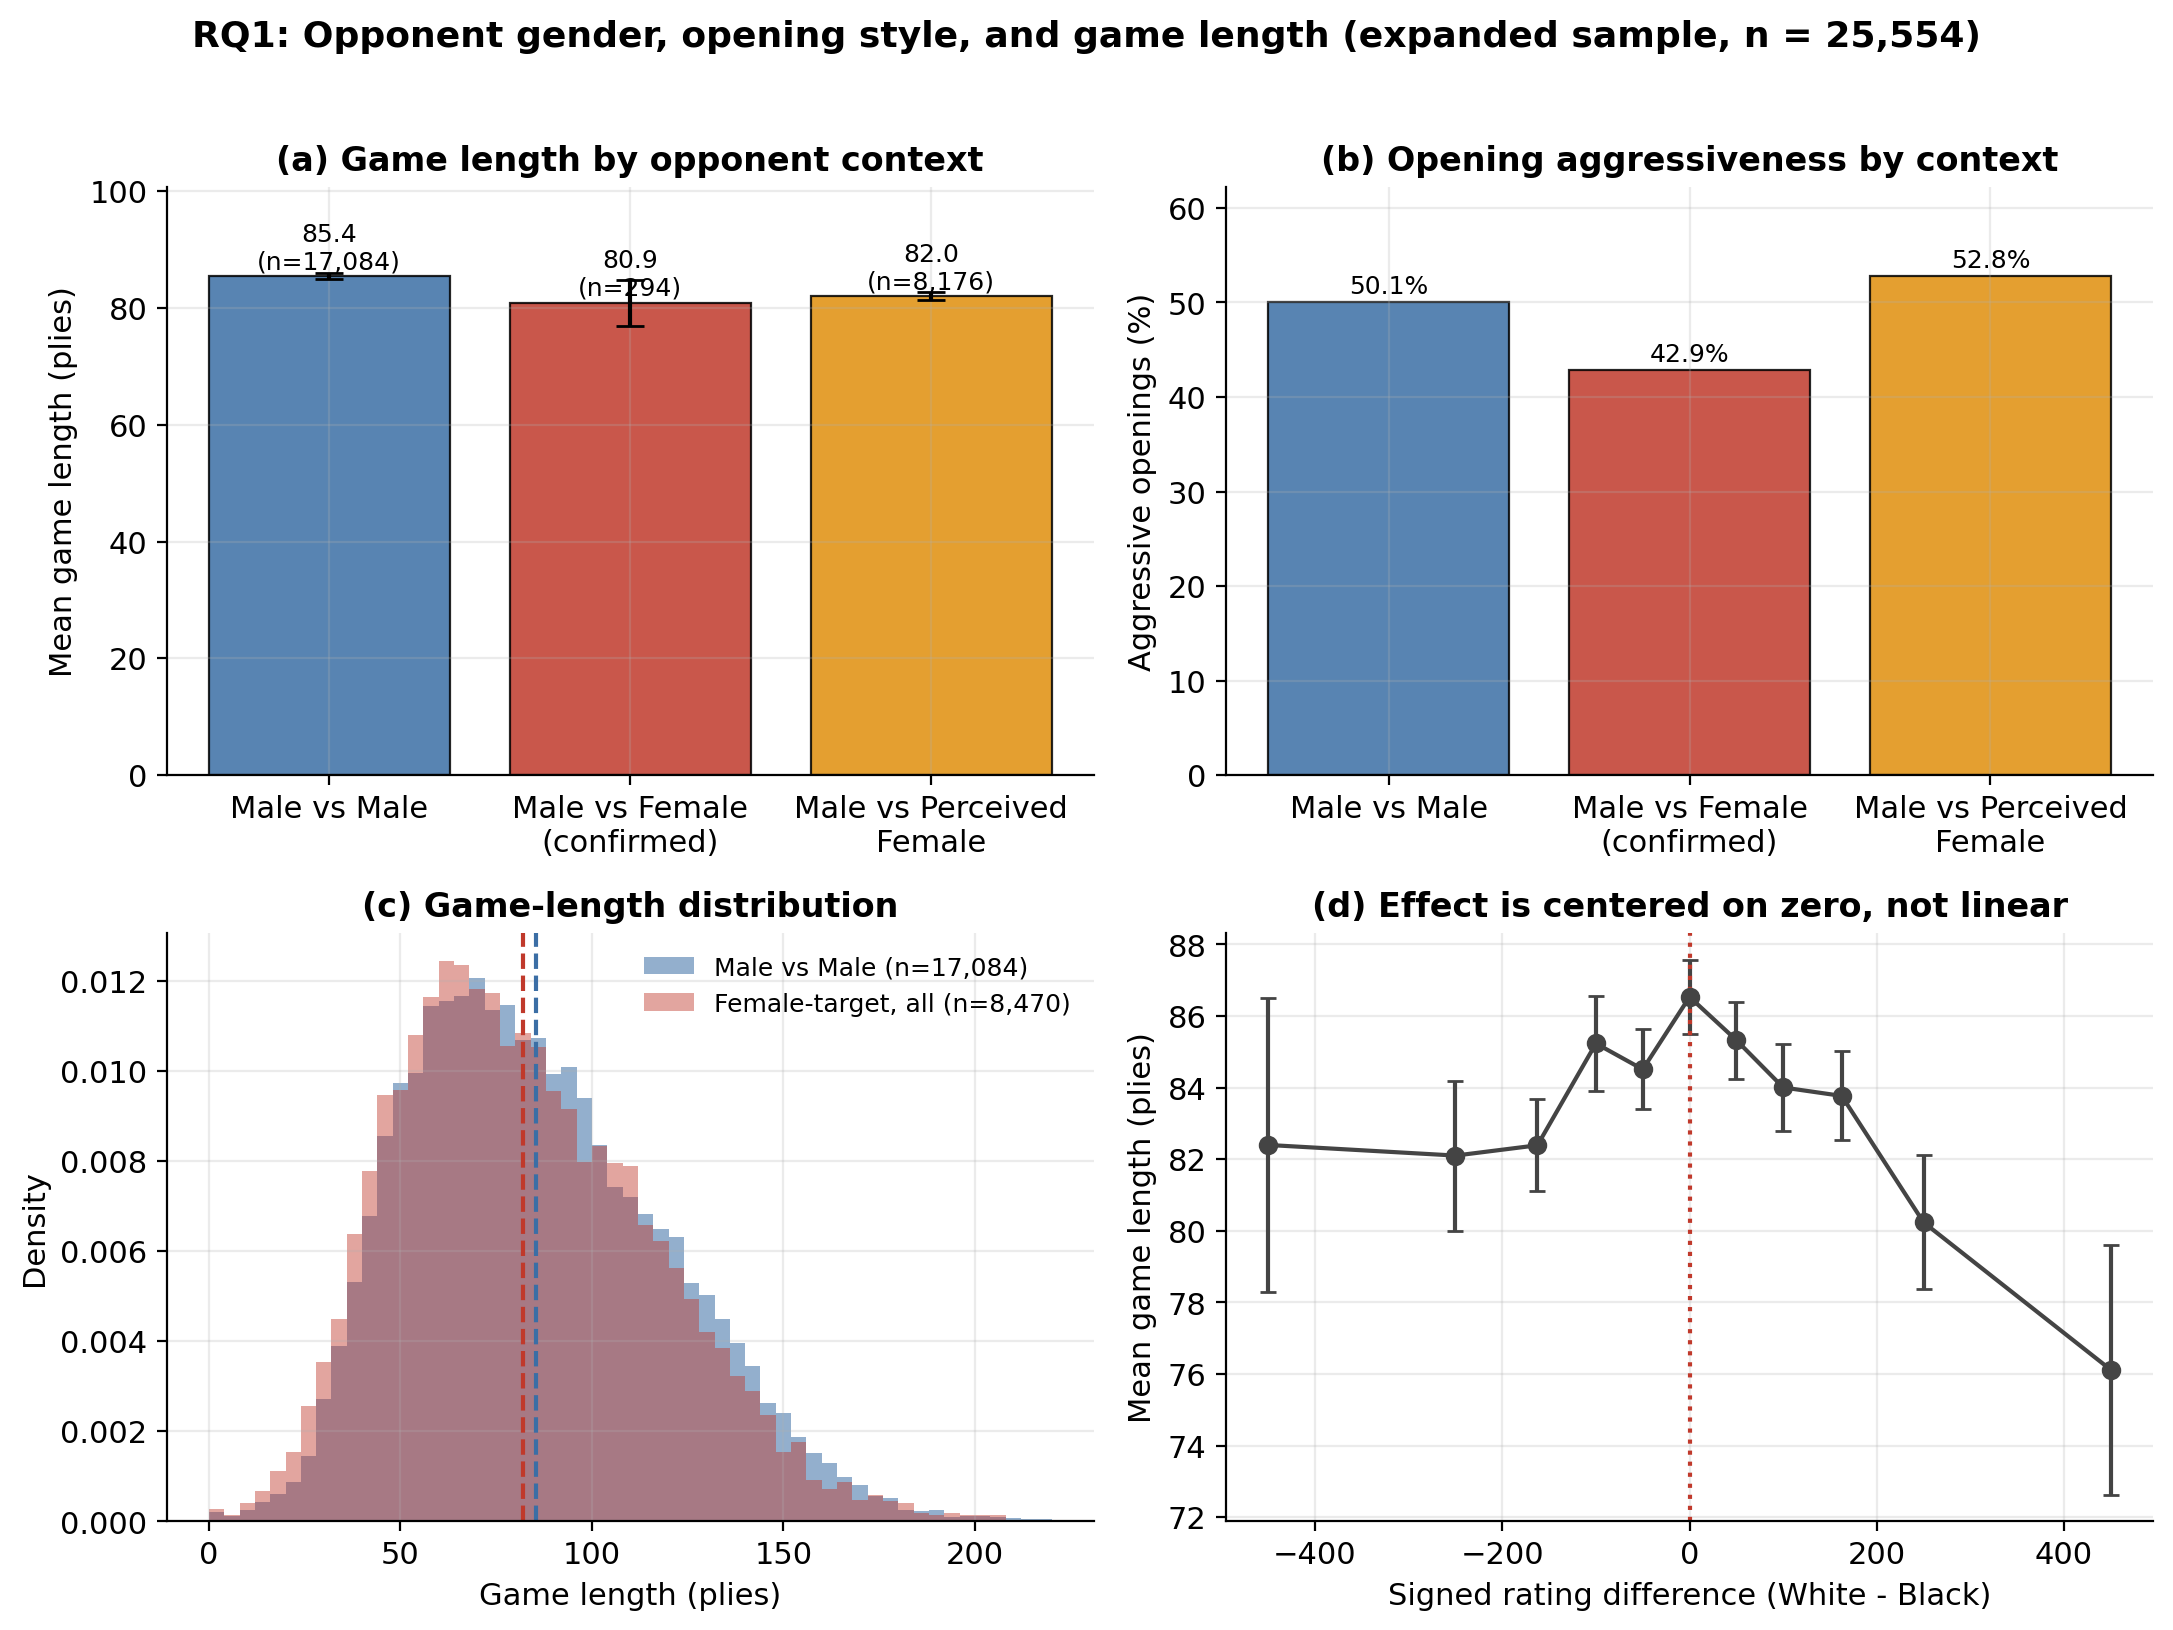
\includegraphics[width=0.97\linewidth]{fig1_rq1_overview.png}
\caption{Expanded RQ1 analysis ($n=25{,}554$): (a) mean game length by opponent-gender
context with 95\% confidence intervals; (b) aggressive-opening rate by context; (c)
game-length distribution for female-target vs.\ male-baseline games; (d) mean game length
across signed rating-difference bins. Panel~(d) shows that the rating effect is centered on
zero rather than linear, which motivates using the \emph{absolute} rating difference as a
control (Fig.~\ref{fig:rq1box}).}
\label{fig:rq1}
\end{figure}

\begin{figure}[H]
\centering
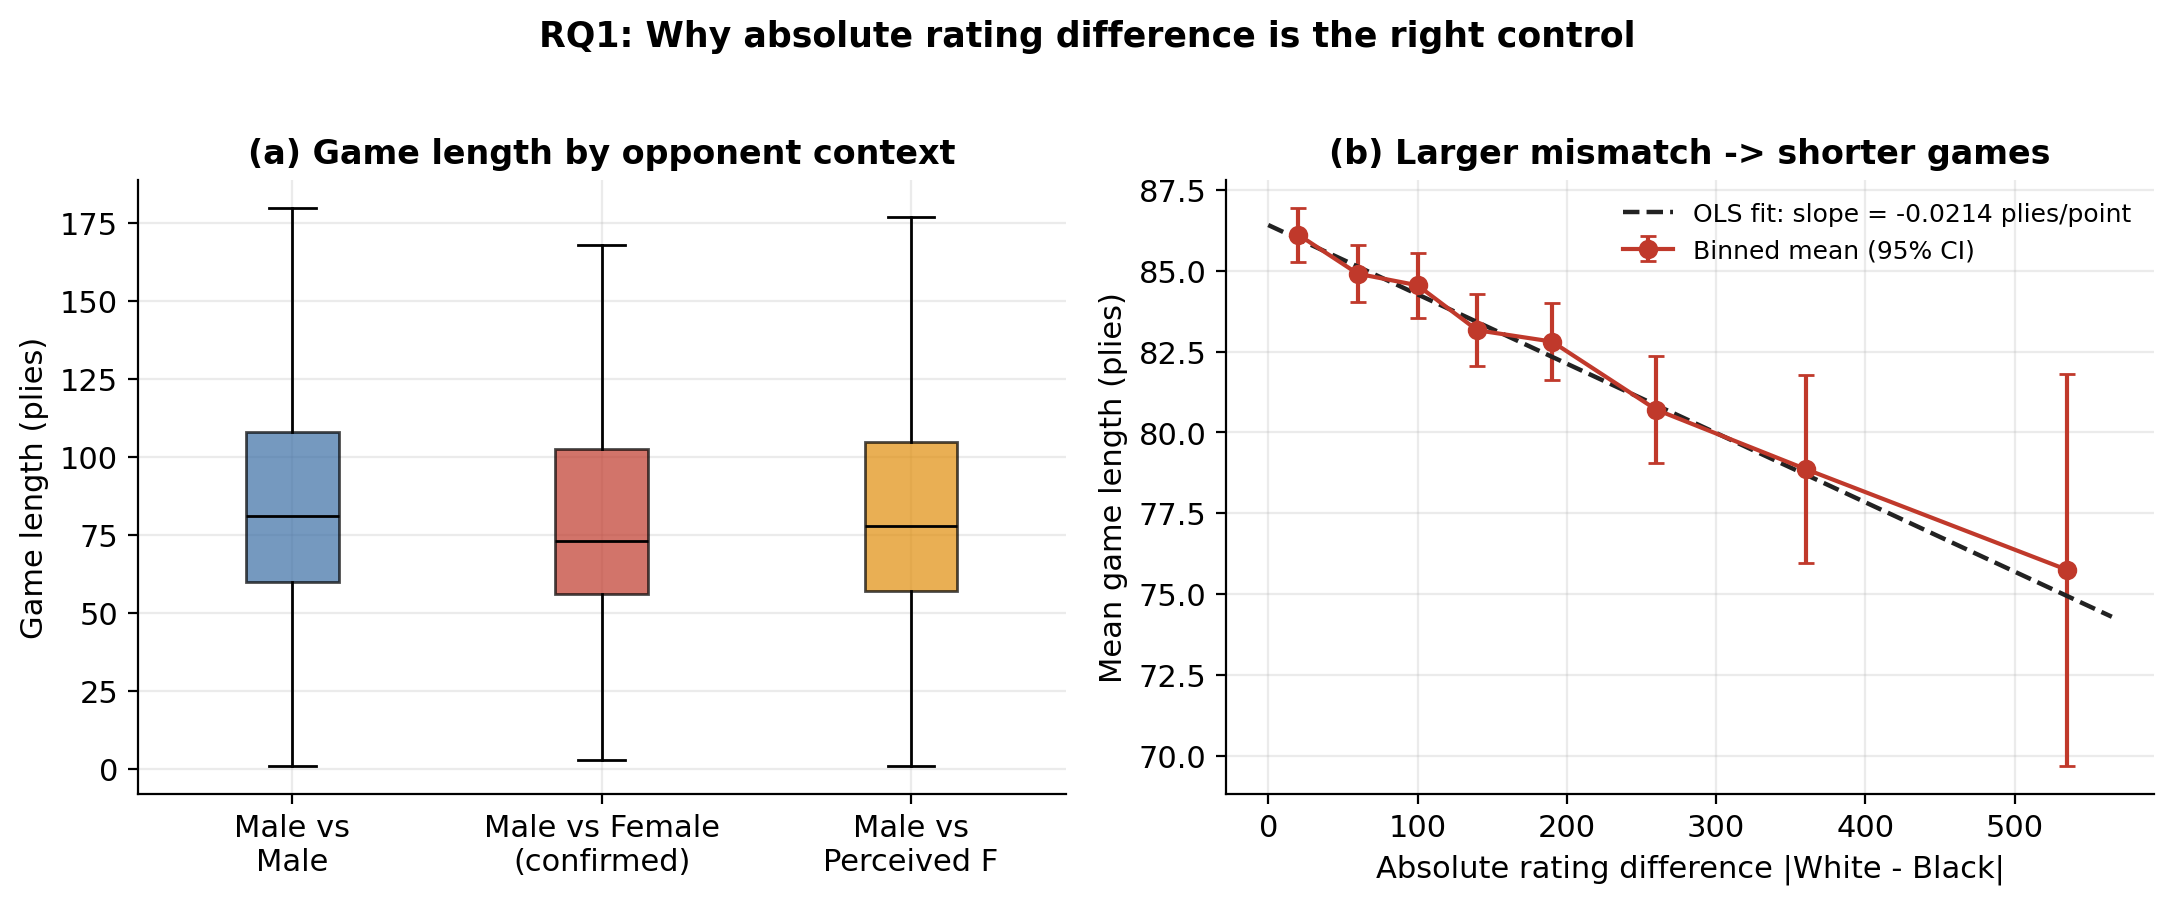
\includegraphics[width=0.96\linewidth]{fig2_rq1_rating_control.png}
\caption{Why the absolute rating difference is the correct control. (a) Game-length
distribution (boxplot) by opponent-gender context. (b) Mean game length declines
monotonically with the \emph{absolute} rating difference (binned means with 95\% CI and an
OLS fit), in contrast to the zero-centered pattern against the signed difference in
Fig.~\ref{fig:rq1}(d).}
\label{fig:rq1box}
\end{figure}

\subsection{RQ2 Results: Rating, Activity, and Opening Style}
\label{sec:rq2res}
The player-level sample contains 729 players (700 male, 29 female), all of whom resolve to
Lichess in this feature table; platform is therefore constant and omitted from
Eq.~\eqref{eq:rq2}.

\paragraph{Correlations.}
Diversity correlates positively with rating for both groups (male $r=0.293$, $p<0.001$;
female $r=0.620$, $p<0.001$). Aggressiveness correlates weakly and non-significantly with
rating (male $r=-0.072$, $p=0.057$; female $r=0.227$, $p=0.235$).

\paragraph{Multivariable regression.}
Table~\ref{tab:rq2reg} reports both models with full diagnostics.

\begin{table}[H]
\caption{RQ2 regressions (player level). Standard errors in parentheses. Predictors:
standardized rating, female indicator, and $\log$(games). Platform omitted (constant =
Lichess). $n=729$.}
\label{tab:rq2reg}
\centering
\begin{tabular}{lcc}
\toprule
Predictor & Aggressiveness & Diversity (Shannon) \\
\midrule
Intercept ($\alpha_0$)   & $0.3994^{***}$ (0.0185) & $1.5488^{***}$ (0.0799) \\
StdRating                & $-0.0106^{*}$ (0.0050)  & $0.1059^{***}$ (0.0218) \\
Female                   & $0.0015$ (0.0249)       & $0.0927$ (0.1078) \\
$\log$(games)            & $0.0072$ (0.0037)       & $0.3601^{***}$ (0.0160) \\
\midrule
$R^2$                    & 0.0089                  & 0.4662 \\
Adjusted $R^2$           & 0.0048                  & 0.4640 \\
$F$ statistic            & 2.16                    & 211.10 \\
$p(F)$                   & 0.092                   & $2.1\times10^{-98}$ \\
\bottomrule
\end{tabular}

\vspace{2pt}
{\footnotesize $^{*}\,p<0.05$, $^{**}\,p<0.01$, $^{***}\,p<0.001$.}
\end{table}

\paragraph{Interpretation.}
Diversity is the most conclusive opening-related result: activity ($\log$ games) is the
dominant driver ($p<10^{-80}$), with rating a strong secondary driver, and together they
explain about 47\% of the variance. In both models the \emph{gender} coefficient is small and
not statistically significant ($p=0.95$ for aggressiveness, $p=0.39$ for diversity), so
opening style is shaped by strength and activity rather than by gender. The aggressiveness
model explains little variance ($R^2=0.009$; overall $F$ not significant), so we treat
aggressiveness as a weak, exploratory signal and diversity as the mature RQ2 finding. Two
caveats temper the gender comparison: the female subsample is small ($n=29$), and the higher
female diversity--rating correlation should not be over-interpreted given that width.

\begin{figure}[H]
\centering
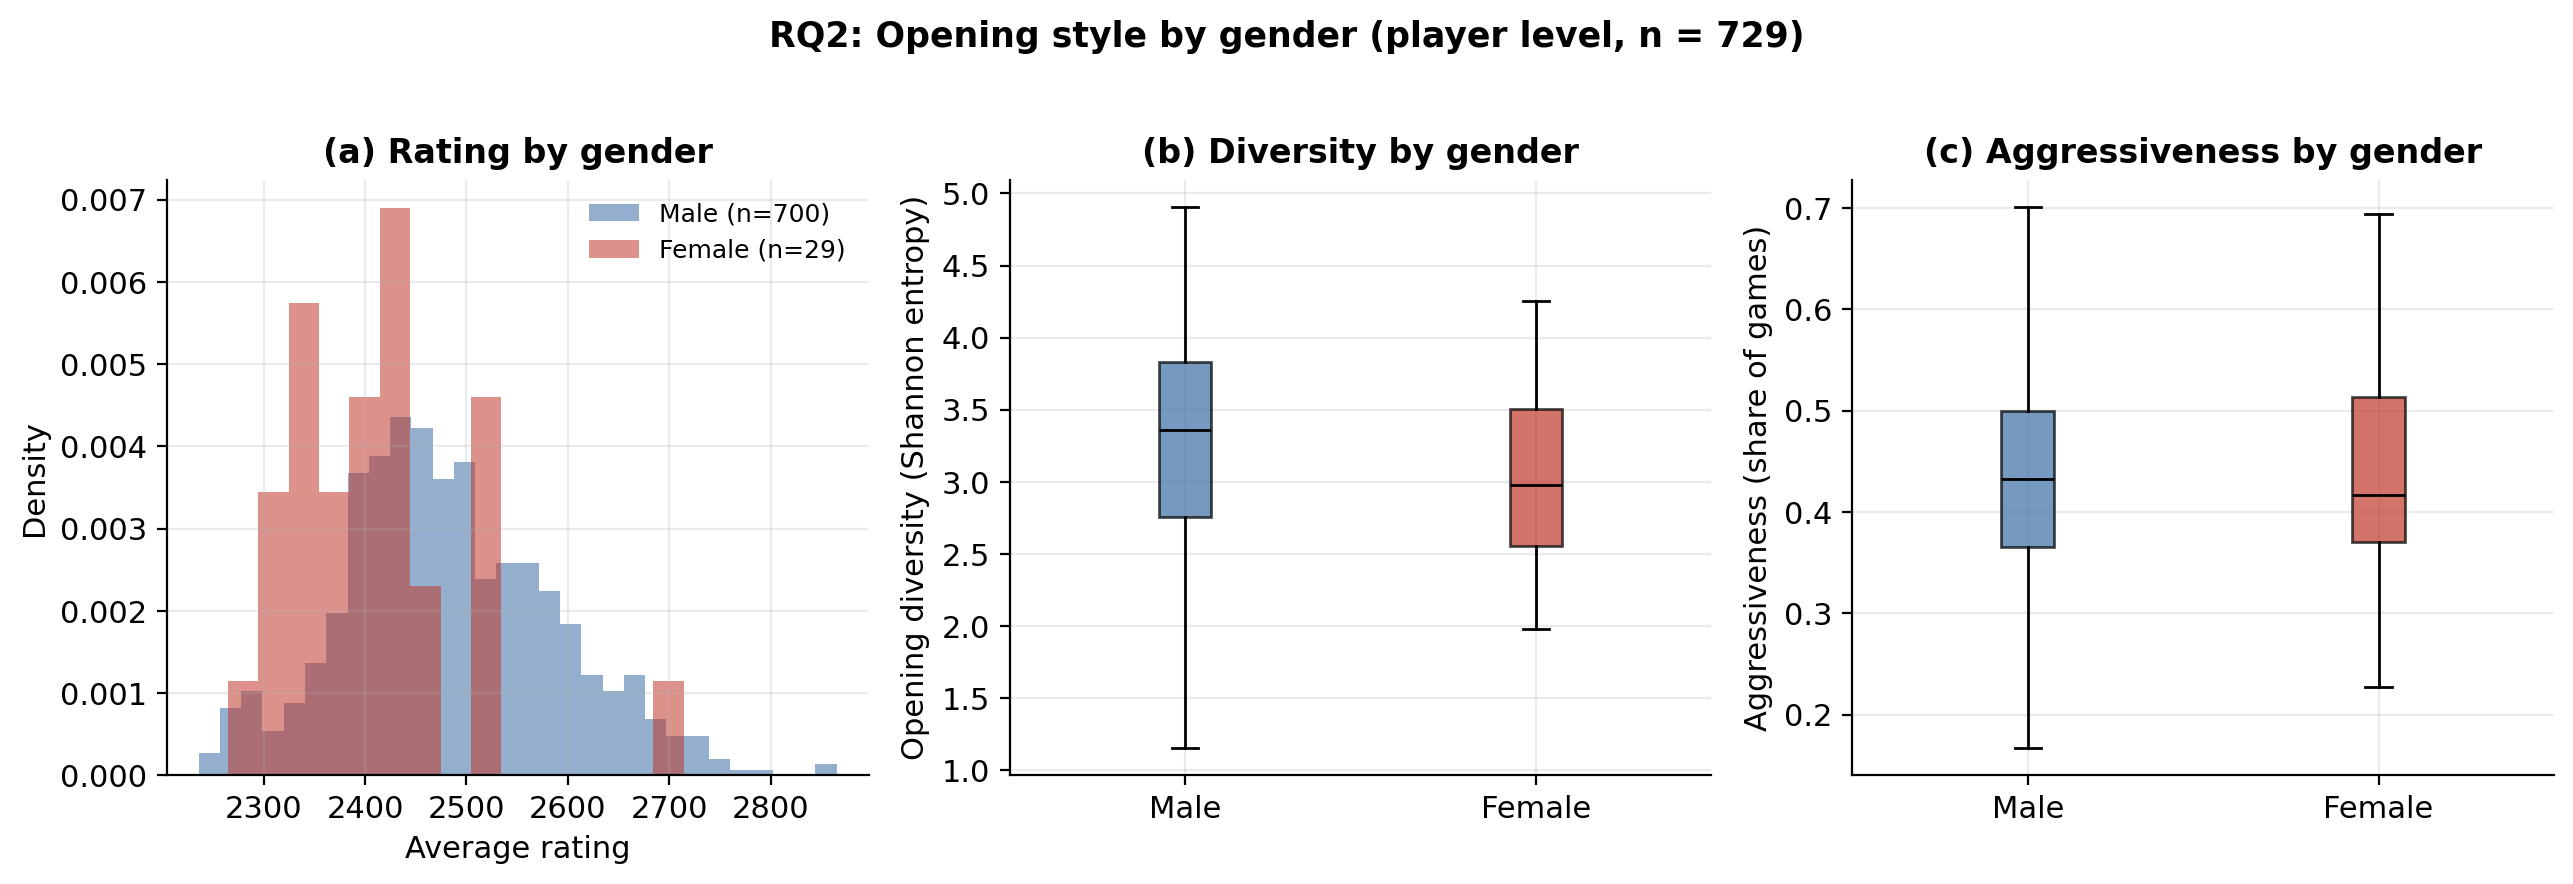
\includegraphics[width=0.98\linewidth]{fig3_rq2_overview.png}
\caption{RQ2 opening style by gender (player level, $n=729$): (a) rating distribution,
(b) opening diversity (Shannon entropy), and (c) opening aggressiveness.}
\label{fig:rq2}
\end{figure}

\begin{figure}[H]
\centering
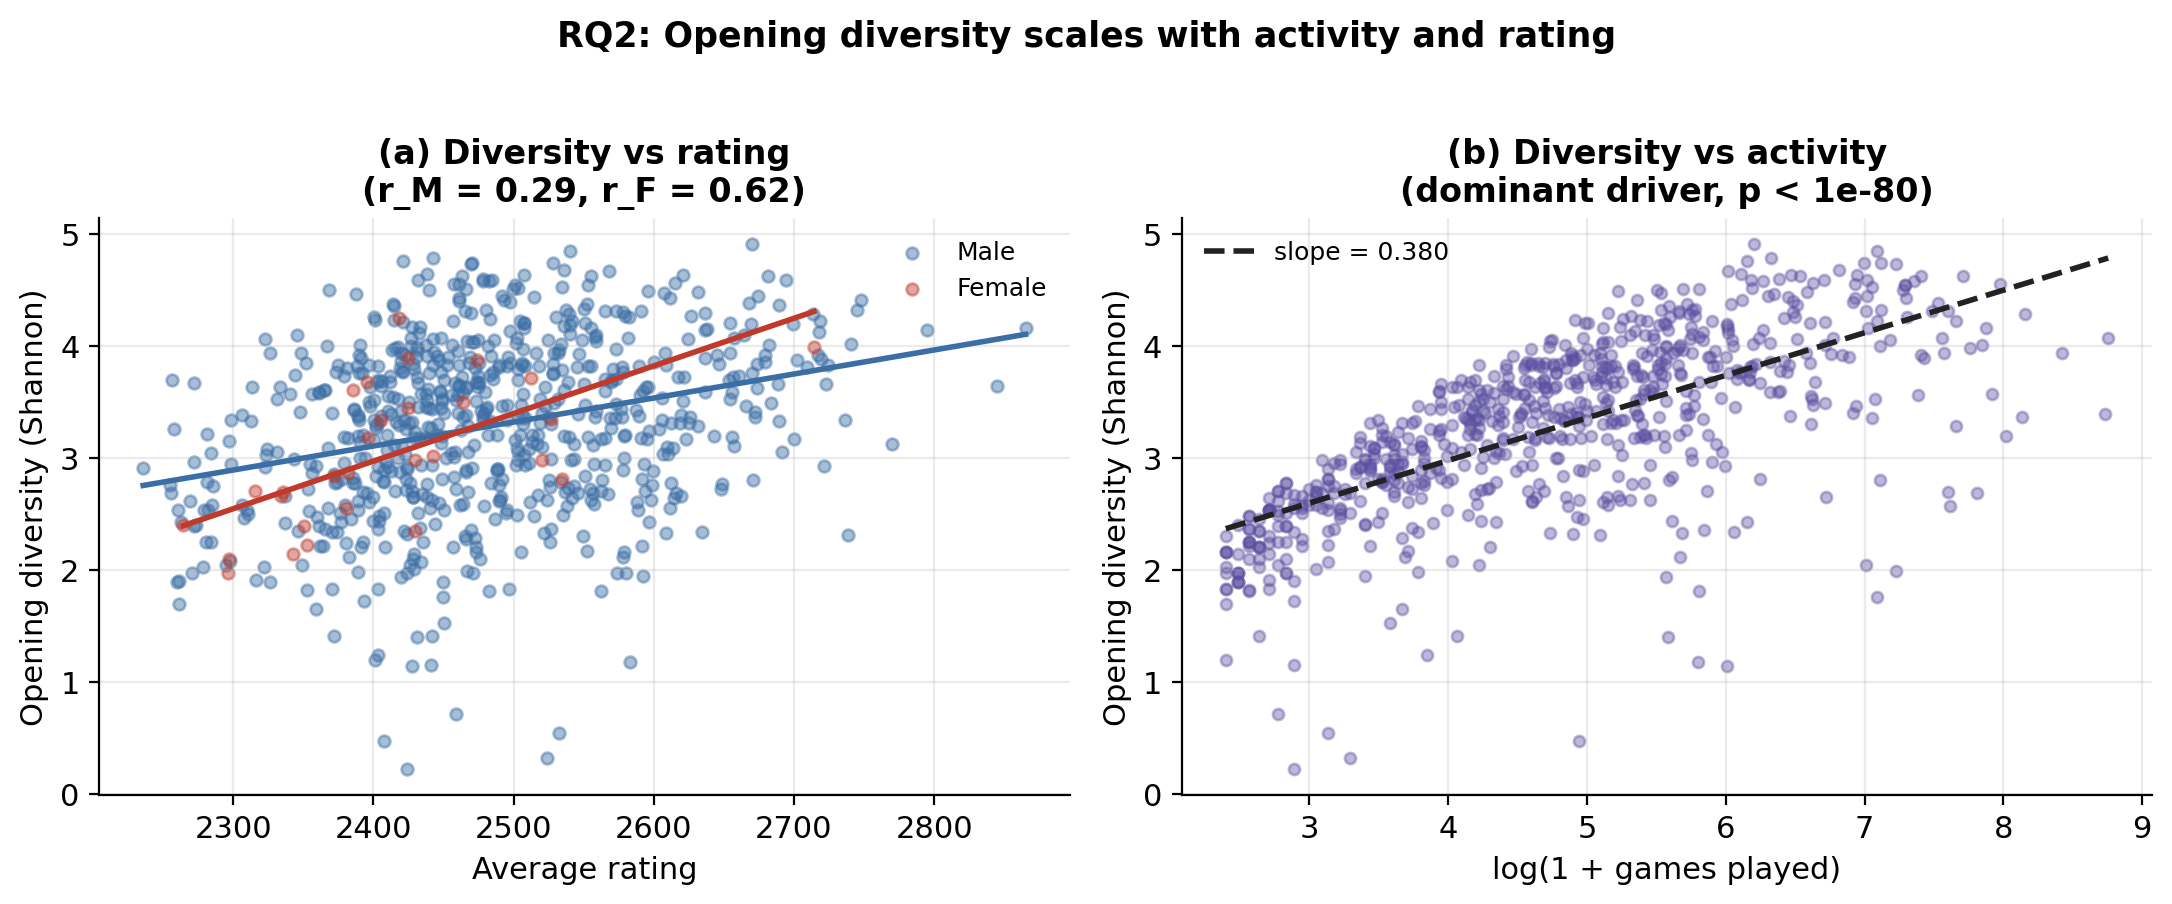
\includegraphics[width=0.95\linewidth]{fig4_rq2_diversity_drivers.png}
\caption{Drivers of opening diversity. (a) Diversity vs.\ average rating with per-gender
linear fits ($r_{\text{male}}=0.29$, $r_{\text{female}}=0.62$). (b) Diversity vs.\ activity
($\log$ games), the dominant predictor in the regression ($p<10^{-80}$).}
\label{fig:rq2div}
\end{figure}

% ============================================================
\section{Discussion}
% ============================================================
\paragraph{What the results say.}
For RQ1, players do not behave identically against female-target opponents: games are
modestly but reliably shorter, with a small shift toward aggressive openings. The effect
survives controls for opening style and --- importantly --- for the \emph{absolute} rating
mismatch, which we showed is the correct rating control. For RQ2, opening diversity is
strongly tied to a player's activity and strength, while gender adds no significant
explanatory power; opening aggressiveness is only weakly explained by the current feature
set.

\paragraph{Why the RQ1 model has low $R^2$, and what is missing.}
A low $R^2$ with a highly significant coefficient simply means the predictor reliably shifts
the mean by a small amount while most of the variance lies elsewhere. Plausible missing
predictors include: time control (bullet/blitz/rapid) and per-move clock data; opening-theory
depth and whether a line is forcing; player-specific tendencies (fixed effects); engine
preparation; rating tier interactions; and game importance. Adding clock and ACPL features is
the most promising route to a better-specified behavioral model. We also stress
\emph{association, not causation}: these regressions identify conditional correlations, not
causal effects.

\subsection{Limitations}
The database is well suited to elite \emph{online} analysis but is not globally
representative of all chess players. Perceived-gender labels are probabilistic and may
misclassify; we mitigate this by separating confirmed from perceived groups, but residual
error remains. Cross-platform linkage is name-based, which can both miss true matches and, in
rare cases, over-merge common names. The RQ2 player sample is Lichess-only and the female
subsample is small ($n=29$). Several models have low explanatory power despite statistical
significance, so practical effect sizes must be read alongside $p$-values.

\subsection{Future Work}
Planned extensions are: (i) engine-based move-quality (ACPL) and per-phase time-allocation
features to give RQ1 a direct decision-quality channel; (ii) FIDE-ID--verified cross-platform
linkage to replace name-only matching; (iii) robustness checks across time-control, platform,
and rating strata, and across title-based vs.\ broader-player samples; and (iv) extending the
RQ2 feature set so aggressiveness can be modeled as reliably as diversity.

% ============================================================
\section{Conclusion}
% ============================================================
The project's central contribution is a reproducible unified database linking FIDE,
Chess.com, and Lichess, which we argue is a research challenge in its own right. Using it, RQ1
shows that female-target contexts correspond to shorter games and a small shift toward
aggressive openings, even after controlling for opening style and absolute rating difference;
the behavioral direction is robust though small in practical size. RQ2 shows that opening
diversity is clearly driven by player activity and strength, with gender playing no
significant role, while aggressiveness remains weakly explained. Together these analyses
demonstrate that the unified database makes principled, controlled behavioral analysis of
elite online chess feasible.

% ============================================================
\section*{Supplementary Information}
% ============================================================
\subsection*{Figure Index}
All figures in this manuscript are generated from the analysis data by
\texttt{figures/make\_figures.py} and stored in \texttt{figures/}:
{\footnotesize\ttfamily
\begin{itemize}\setlength\itemsep{0pt}
  \item fig1\_rq1\_overview.png \quad(Fig.~\ref{fig:rq1})
  \item fig2\_rq1\_rating\_control.png \quad(Fig.~\ref{fig:rq1box})
  \item fig3\_rq2\_overview.png \quad(Fig.~\ref{fig:rq2})
  \item fig4\_rq2\_diversity\_drivers.png \quad(Fig.~\ref{fig:rq2div})
\end{itemize}}
Additional exploratory plots from the pipeline are available under
\texttt{analysis/plots/} and \texttt{results/plots/}.

\subsection*{Reproducibility}
{\footnotesize
Core scripts:
\begin{itemize}\setlength\itemsep{0pt}\ttfamily
  \item analysis/05\_comprehensive\_lichess\_extraction.py
  \item analysis/06\_rq1\_expanded\_analysis.py
  \item analysis/02\_rq2\_opening\_repertoire\_analysis.py
  \item analysis/07\_comprehensive\_statistics\_report.py
\end{itemize}
Key generated outputs:
\begin{itemize}\setlength\itemsep{0pt}\ttfamily
  \item data/rq1\_analysis\_expanded.csv
  \item analysis/games\_male\_vs\_perceived\_female.csv
  \item analysis/rq1\_expanded\_results.csv
  \item analysis/rq2\_regression\_results.csv
  \item analysis/comprehensive\_statistics\_summary.csv
\end{itemize}}
Repository: \url{https://github.com/sajayshenoy/Masters-Project}.

% ============================================================
\begin{thebibliography}{9}

\bibitem{bilalic2009why}
M.~Bilali\'c, K.~Smallbone, P.~McLeod, and F.~Gobet,
``Why are (the best) women so good at chess? Participation rates and gender differences in
intellectual domains,'' \emph{Proceedings of the Royal Society B: Biological Sciences},
vol.~276, no.~1659, pp.~1161--1165, 2009.

\bibitem{blanch2017sex}
A.~Blanch,
``Sex differences in chess performance: Analyzing participation rates, age, and practice,''
\emph{Personality and Individual Differences}, vol.~104, pp.~117--121, 2017.

\bibitem{maass2008checkmate}
A.~Maass, C.~D'Ettole, and M.~Cadinu,
``Checkmate? The role of gender stereotypes in the ultimate intellectual sport,''
\emph{European Journal of Social Psychology}, vol.~38, no.~2, pp.~231--245, 2008.

\bibitem{backus2023gender}
P.~Backus, M.~Cubel, M.~Guid, S.~S\'anchez-Pag\'es, and E.~L\'opez Ma\~nas,
``Gender, competition, and performance: Evidence from chess players,''
\emph{Quantitative Economics}, vol.~14, no.~1, pp.~1--33, 2023.

\end{thebibliography}

\end{document}
